\section{Minimal Span-based CKY Parsing Framework}
\label{sec:phr:cky-based}

Let us now see our phrasal-anchoring parser for UCCA. We introduce
the transformation we used to reduce UCCA parsing into a consituent
parsing task, and finally introduce the detailed CKY model for the
constituent parsing.


\subsection{Graph-to-CT Transformation}
\label{ssec:phr:graph-ct}

We propose to transform a graph into a constituent tree structure for
parsing, which is also used in recent work~\cite{jiang2019hlt}.
Figure~\ref{fig:ucca-to-CT} shows an example of transforming a UCCA
graph into a constituent tree. The primary transformation assigns the
original label of an edge to its child node. Then to make it
compatible with parsers for standard PennTree Bank format, we add some
auxiliary nodes such as special non-terminal nodes, TOP, HEAD, and
special terminal nodes TOKEN and MWE. We remove all the ``remote''
annotation in UCCA since the constituent tree structure does not
support reentrance.  A fully compatible transformation should support
both graph-to-tree and tree-to-graph transformation.

In our case, due to time constraints, we remove those remote edges and
reentrance edges during training. Besides that, we also noticed that
for multi-word expressions, the children of a parent node might not be
in a continuous span (i.e., discontinuous constituent), which is also
not supported by our constituent tree parser. Hence, when training the
tree parser, by reattaching the discontinuous tokens to its nearest
continuous parent nodes, we force every sub span are continuous in the
transformed trees. We leave the postprocessing to recover those
discontinuous as future work.

For inference, given an input sentence, we first use the trained
constituent tree parsing model to parse it into a tree, and then we
transform a tree back into a directed graph by assigning the edge
label as its child's node label, and deleting those auxiliary labels,
adding anchors to every remaining node.

\begin{figure}[!h]
\centering
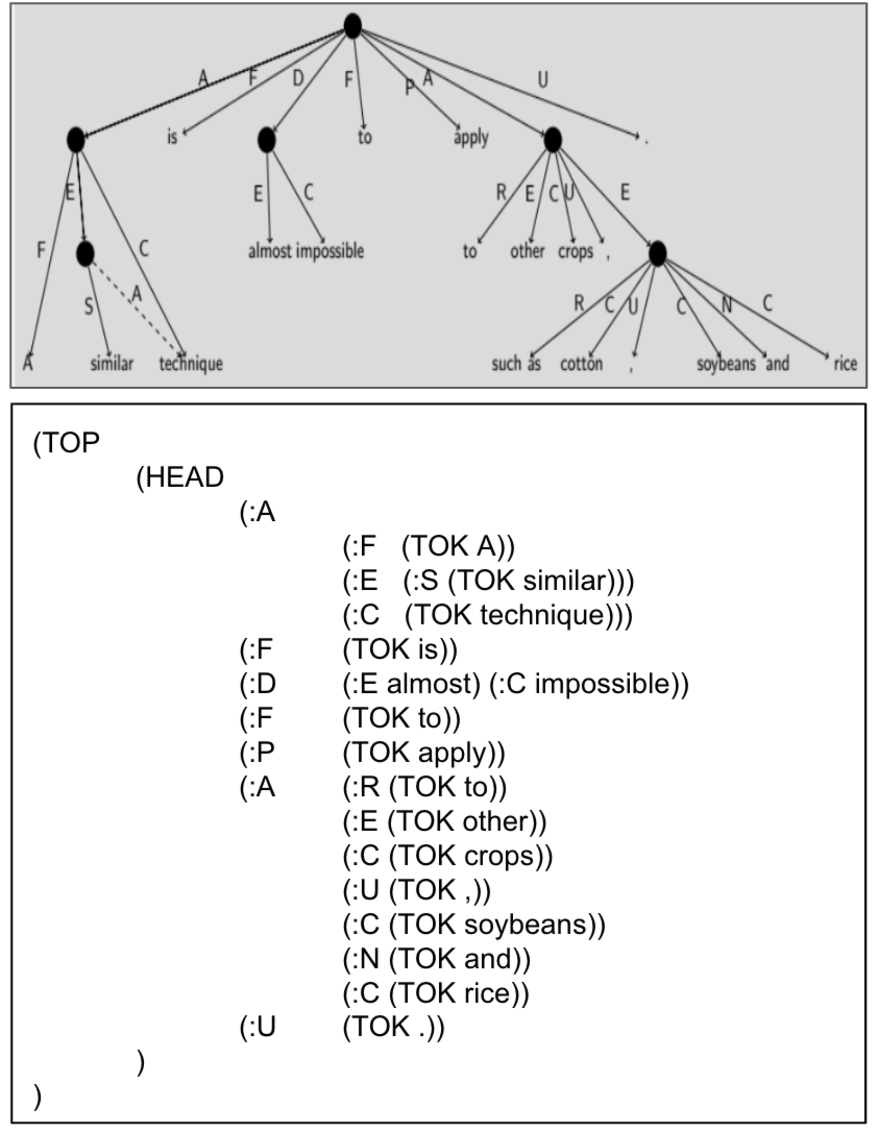
\includegraphics[width=0.48\textwidth]{ucca-to-CT.pdf}
\caption{\label{fig:ucca-to-CT} UCCA to Constituent Tree Transformation for [wsj\#0209013]}
\end{figure}


\subsection{CKY Parsing}
\label{ssec:phr:cky}
After transforming the UCCA graph into a constituent tree, we reduce
the UCCA parsing into a constituent tree parsing problem. Similar to
the previous work on UCCA constituent tree
parsing~\cite{jiang2019hlt}, we use a minimal span-based CKY parser
for constituent tree parsing.  The intuition is to use dynamic
programming to recursively split the span of a sentence recursively,
as shown in Figure~\ref{fig:ucca-to-CT}. The entire sentence can be
splitted from top to bottom until each span is a single unsplittable
tokens. For each node, we also need to assign a label. Two simplified
assumptions are made when predicting the hole tree given a
sentence. However, different with previous work, we use 8-layers with
8 heads transformer encoder, which shows better performance than LSTM
in \citet{kitaev2018constituency}.

\paragraph{Tree Factorization} In the graph-to-tree transformation, we
move the edge label to its child node. By assuming the labels for each
node are independent, we factorize the tree structure prediction as
independent span-label prediction as Equation
\ref{eq:tree_factorize}. However, this assumption does not hold for UCCA.
Please see more error analysis in \S \ref{ssec:error_breakdown}

\begin{equation}
  \label{eq:tree_factorize}
 \begin{aligned} T^{*}  & = \underset{T}{\textbf{arg\,max}} s(T)     \\ s(T)
                        & = \sum_{(i,j,l) \in T} s(i,j,l)
\end{aligned}
\end{equation}

\paragraph{CKY Parsing} By assuming the label prediction is
independent of the splitting point, we can further factorize the whole
tree as the following dynamic programming in Equation \ref{eq:tree_chart}.

\begin{equation}
  \label{eq:tree_chart}
\begin{aligned}
      s_{\text{best}}(i, i+1) & = \underset{l}{\textbf{max}} s(i,i+1, l) \\
      s_{\text{best}}(i, j) & = \underset{l}{\textbf{max}} s(i,j, l)
      \\ & + \underset{k}{\textbf{max}}[ s_{\text{best}}(i,k) +
      s_{\text{best}}(k,j) ]
\end{aligned}
\end{equation}

\subsection{Span Encoding}
\label{ssec:phr:span}

For each span $(i,j)$, we represent the span encoding vector
$v_{(i,j)} = [\vec{y_{j}} - \vec{y_{i}}] \oplus [\cev{y_{j+1}} -
\cev{y_{i+1}}] $. $\oplus$ denotes vector concatenation. Assuming a
bidirectional sentence encoder, we use the forward and backward
encodings $\vec{y_{i}}$ and $\cev{y_{i}}$ of $i_{th}$ word. Following
the previous work, and we also use the loss augmented inference
training. More details about the network
architecture are in the Section \ref{ssec:exp_setup}

% TODO: try it on EDS to get a result, leave as future work

%%% Local Variables:
%%% mode: latex
%%% TeX-master: "../thesis-main.ltx"
%%% End:
